\section{Methods}

\subsection{Tooling}
A lot of tooling is available for use in software development. We have chosen a set of tooling that we would like to use for this project. In this section we will explain the selection of tooling.

\paragraph{Telegram}
~\\ The chat application Telegram will be used to communicate with the group (or specific members of the group). A group chat will be created so that messages can be quickly shared with the group.

\paragraph{GitHub}
~\\ Git will be used as the source control system. All code (and documents) will be put inside a GitHub repository. Branches will be made for all changes and reviews will be done when a Pull Request is opened.

GitHub has a relatively new feature called "projects". A GitHub project consists of columns containing GitHub issues. This looks very similar to a tool called Trello. An example can be seen in \cref{fig:githubproject}. Since we will use GitHub quite extensively, we will use a GitHub project as our product backlog.

\begin{figure}
    \centering
    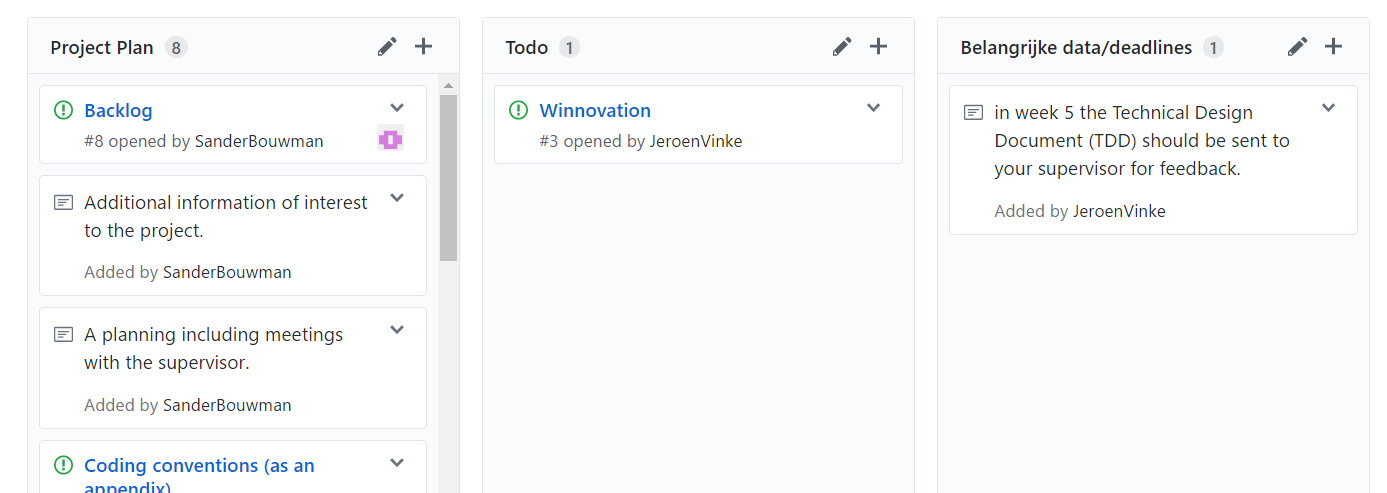
\includegraphics[scale=0.75]{images/github-projects.PNG}
    \caption{GitHub project}\label{fig:githubproject}
\end{figure}

\paragraph{Editors}
~\\ The group will use either Visual Studio or the Sealion editor (depending on personal preference). 

\paragraph{TravisCI}
~\\ Since all our code is in a public GitHub repository, we can easily configure a build service using TravisCI. This build server will compile the game, run the linter and the unit tests. This will probably make the review process quicker.
 


